\documentclass[a4paper,12pt,oneside]{report}

\usepackage[T1]{fontenc} % caractères accentués
\usepackage[utf8]{inputenc} % codage
\usepackage[hidelinks]{hyperref} % faire disparaître le carré bleu autour les liens
\usepackage{graphicx} % images
\usepackage{geometry} % setter le margin du document
\usepackage{fancyhdr} % header et footer du document
\usepackage[toc]{glossaries} % glossaire
\usepackage{setspace} % espace entre les lignes
\usepackage{tocloft} % style de la table des matières
\usepackage{enumitem}
\usepackage{tabularx}
\usepackage{longtable}
\usepackage[underline=true,rounded corners=false]{pgf-umlsd}

\usepackage{listings}
\usepackage{color}

\onehalfspacing

\graphicspath{{images/}}

\renewcommand{\contentsname}{Table des matières}
\renewcommand{\chaptername}{Chapitre}
\renewcommand*\glossarypreamble{\thispagestyle{glossary}}

\geometry{hmargin=3.5cm,vmargin=3.5cm,lmargin=2cm,rmargin=2cm}

\tocloftpagestyle{summary}

\fancypagestyle{cover} {

	% head
	\fancyhead[L]{Univ. Lille 1, Master 1 Informatique}
	\fancyhead[R]{2014 -- 2015}

	% foot
	\renewcommand{\footrulewidth}{0.8pt}
	\fancyfoot[R]{\includegraphics[width=\textwidth, height=2.9cm]{images/footer.jpg}}

}

\fancypagestyle{summary} {

	% head
	\fancyhead[L]{\leftmark}
	\fancyhead[R]{~}
	
	% foot
	\renewcommand{\footrulewidth}{0.8pt}
	\fancyfoot[L]{\textsc{GROUPE ASMA}}
	\fancyfoot[C]{\textsc{SUIVI DE PROJET}}
	\fancyfoot[R]{\textsc{Page \thepage}}

}

\fancypagestyle{document} {

	% head
	\fancyhead[L]{\leftmark}
	\fancyhead[R]{\rightmark}

	% foot
	\renewcommand{\footrulewidth}{0.8pt}
	\fancyfoot[L]{\textsc{GROUPE ASMA}}
	\fancyfoot[C]{~}
	\fancyfoot[R]{\textsc{Page \thepage}}

}

\fancypagestyle{introduction} {
	
	% head
	\fancyhead[L]{\textsc{INTRODUCTION}}
	\fancyhead[R]{~}

	% foot
	\renewcommand{\footrulewidth}{0.8pt}
	\fancyfoot[C]{~}
	\fancyfoot[R]{\textsc{Page \thepage}}
}

\fancypagestyle{glossary} {

	% head
	\fancyhead[L]{\textsc{GLOSSAIRE MÉTIER}}
	\fancyhead[R]{~}

	% foot
	\renewcommand{\footrulewidth}{0.8pt}
	\fancyfoot[L]{\textsc{GROUPE ASMA}}
	\fancyfoot[C]{~}
	\fancyfoot[R]{\textsc{SUIVI DE PROJET}}

}


\makeglossaries
\thispagestyle{glossary}

\newglossaryentry{hypermarche} {
    name=hypermarché,
    description={un hypermarché est un commerce de détail en libre-service, de grande taille (définie en France par une surface égale ou supérieure à 2 500 m2.}
}

\newglossaryentry{douchette} {
	name=douchette,
	description={représente un lecteur de code-barres, permet de lire les informations stockées sous la forme de codes-barres ou QRCode.}
}

\newglossaryentry{code_barres} {
	name=code-barres,
	description={représente une donnée numérique ou alphanumérique sous forme d'un symbole constitué de barres et d'espaces dont l'épaisseur varie en fonction de la symbologie utilisée et des données ainsi codées.}
}

\newglossaryentry{qr_code} {
	name=QR Code,
	description={un type de code-barres en deux dimensions constitué de modules noirs disposés dans un carré à fond blanc. L'agencement de ces points définit l'information que contient le code. QR (abréviation de Quick Response) signifie que le contenu du code peut être décodé rapidement après avoir été lu par un lecteur de code-barres, un téléphone mobile, un smartphone, ou encore une webcam. Son avantage est de pouvoir stocker plus d'informations qu'un code à barres, et surtout des données directement reconnues par des applications, permettant ainsi de déclencher facilement des actions.}
}

\newglossaryentry{gamme} {
	name=gamme,
	description={une gamme de produits est généralement définie comme un ensemble de produits de même catégorie ou répondant au même type de besoin proposé par une même marque ou fabricant.}
}

\newglossaryentry{smartphone} {
	name=smartphone,
	description={un smartphone, ordiphone ou téléphone intelligent, est un téléphone mobile évolué disposant des fonctions d'un assistant numérique personnel, d'un appareil photo numérique et d'un ordinateur portable. Il peut exécuter divers logiciels/applications grâce à un système d'exploitation}
}

\newglossaryentry{caddie} {
	name=caddie,
	description={un chariot, métallique ou en matière plastique, conçu pour faciliter le transport des marchandises achetées dans un supermarché ou d'autres types de magasins. (remarque : Caddie est une marque déposé par une société anonyme patronyme)}
}

\newglossaryentry{robot} {
	name=robot,
	description={Un robot est un dispositif mécatronique (alliant mécanique, électronique et informatique) accomplissant automatiquement soit des tâches qui sont généralement dangereuses, pénibles, répétitives ou impossibles pour les humains, soit des tâches plus simples mais en les réalisant mieux que ce que ferait un être humain.}
}

\newglossaryentry{tablette_interactive} {
	name=tablette interactive,
	description={fait référence à une tablette de grande taille (environ la surface d’un téléviseur de salon). Un ordinateur portable ultraplat qui se présente sous la forme d'un écran tactile sans clavier et qui offre à peu près les mêmes fonctionnalités qu'un ordinateur personnel.}
}

\newglossaryentry{Wifi} {
	name=Wifi,
	description={Le Wifi est un ensemble de protocoles de communication sans fil régis par les normes du groupe IEEE 802.11 (ISO/CEI 8802-11). Un réseau Wifi permet de relier sans fil plusieurs appareils informatiques (ordinateur, routeur , smartphone, décodeur Internet, etc.) au sein d'un réseau informatique afin de permettre la transmission de données entre eux.}
}

\newglossaryentry{GPS} {
	name=GPS,
	description={Le Global Positioning System (GPS) – que l'on peut traduire en français par « système de localisation mondial » – est un système de géolocalisation fonctionnant au niveau mondial. En 2011, il est avec GLONASS, un système de positionnement par satellites entièrement opérationnel et accessible au grand public.}
}

\newglossaryentry{NFC} {
	name=NFC,
	description={La communication en champ proche (en anglais near field communication, NFC) est une technologie de communication sans-fil à courte portée et haute fréquence, permettant l'échange d'informations entre des périphériques jusqu'à une distance d'environ 10 cm. Cette technologie est une extension de la norme ISO/CEI 14443 standardisant les cartes de proximité utilisant la radio-identification (RFID), qui combinent l'interface d'une carte à puce et un lecteur au sein d'un seul périphérique. Un périphérique NFC est capable de communiquer avec le matériel ISO/CEI 14443 existant, avec un autre périphérique NFC ou avec certaines infrastructures sans-contact existantes comme les valideurs des transports en commun ou les terminaux de paiement chez les commerçants.}
}


\pagestyle{document}

\begin{document}
	\thispagestyle{cover}

\includegraphics[width=5cm, scale=0.6]{logo_univ.jpg} \hfill \includegraphics[scale=0.6]{logo_ieea.jpg} \\
~\\
\hspace*{0.5cm} {\Large \textit{Université Lille 1}} \hfill {\Large \textit{IEEA}} \hspace*{0.5cm}\\

\vspace*{17mm}

\begin{center}
	\begin{Huge} \underline{Rapport de Travaux Pratiques} \end{Huge}\\[4mm]

	\vspace*{15mm}

	\rule[0.5ex]{\linewidth}{2pt}\vspace*{-\baselineskip}\vspace*{3.2pt}
	\rule[0.5ex]{\linewidth}{1pt}\\[\baselineskip]

		\begin{Huge} \textbf{Algorithmes et ComplexiTé (ACT)} \end{Huge}\\[4mm]
		\begin{Huge} \textbf{TP4 : La classe NP} \end{Huge}\\[4mm]

	\rule[0.5ex]{\linewidth}{1pt}\vspace*{-\baselineskip}\vspace{3.2pt}
	\rule[0.5ex]{\linewidth}{2pt}\\

	\vspace*{20mm}

	{\large \textit{\underline{Auteur :}}} \hfill {\large \textit{\underline{Professeur :}}}\\
	~\\
	{\large Salla DIAGNE} \hfill {\large Sophie TISON}\\
	{\large Anis TELLO} \hfill {\large}
	
	\vspace*{20mm}
	
	{\large\textsc{12 Novembre 2014}}
\end{center}
	\newpage
\thispagestyle{empty}
%\begin{center}
%\vspace*{\stretch{1}}
%\centering
%\textit{Cette page a intentionnellement été laissée vierge.}
%\vspace*{\stretch{1}}
%\end{center}
\newpage
	 \tableofcontents
	\chapter*{Introduction}
	\thispagestyle{introduction}
	\addcontentsline{toc}{chapter}{Introduction}
	Dans ce projet, nous nous sommes focalisés sur l'expérience client.
	\chapter{Système actuel}
		\thispagestyle{document}
	\chapter{Système proposé}
		\thispagestyle{document}
		\section{Vue d'ensemble}
		\section{Exigences fonctionnelles}
		\section{Exigences non fonctionnelles}
		\section{Modèles}
			\subsection{Scénarios concrets}
\subsubsection{Avec un \gls{smartphone} à l'\gls{hypermarche}}
					José va faire ses courses dans l'\gls{hypermarche} du futur. Il s'arme de son \gls{smartphone} et lance l'application du futur, nommée fDrive.\\
					À l'entrée, il se connecte au réseau \gls{Wifi} de l'\gls{hypermarche} et obtient toutes les nouvelles promotions et nouveaux arrangements du magasin. Puisqu'il a l'habitude d'acheter les mêmes articles chaque semaine, José consulte son historique d'achats et sélectionne ce qu'il désire se procurer à nouveau.\\
					Il veut aussi tester une nouvelle \gls{gamme} de shampooing "spéciale crépus" qui vient de faire irruption dans le magasin; il tape le mot "shampooing" dans la barre de recherche de son application et se laisse guider vers le rayon Produits de beauté. L'application fait en sorte de le faire passer par quelques promotions sur des articles déjà achetés auparavant.\\
					Ignorant ces promotions, José court vers le shampooing qu'il désire et flashe son article. La description et le prix de celui-ci s'affichent. Il ajoute le shampooing à son panier et valide ce dernier. L'application lui indique l'endroit où il doit payer. Il se fait guider, à la manière d'un \gls{GPS}, au guichet indiqué.\\
					2 minutes d'attente plus tard, son numéro de commande apparaît sur le guichet. Il paye avec son téléphone et récupère son \gls{caddie} préparé avec soin par un \gls{robot}. Heureux, il repart de l'hypermarché du futur avec la plus grande des satisfactions.
				\subsubsection{Sans \gls{smartphone} à l'\gls{hypermarche}}
					Dartagnan veut faire ses courses. Il a 63 ans, en pleine forme et n'a pas de \gls{smartphone}. Il ne sait pas ce qui il veut acheter, il veut juste voir à quoi ressemble l'\gls{hypermarche} du futur dont tout le monde parle tant.\\
					Il entre dans le magasin et une hôtesse l'accueille pour lui en expliquer le fonctionnement. Comme il n'a pas de \gls{smartphone}, elle lui propose d'utiliser une \gls{douchette} du magasin, nommée fDouchette, pour flasher les articles avec.
					Elle l'accompagne dans le magasin pour lui montrer comment se servir de cette \gls{douchette} : il flashe un article, il peut choisir la quantité, et il peut aussi le supprimer s'il se trompe. Elle lui explique qu'il n'a pas besoin de prendre les articles et les mettre dans un \gls{caddie} car un \gls{robot} se charge de prendre tous les articles pour lui et les lui ramener à la caisse. Dartagnan est content parce qu'il n'a rien à transporter.\\
					Il demande ensuite à l'hôtesse où il peut se procurer des cookies d'une certaine marque, un article qui est devenu rare. L'hôtesse l'ignore mais en profite pour l'emmener voir une des tables interactives disposées dans le magasin tous les 25m. La table permet de rechercher un article, la prix, la description, l'endroit où il peut le trouver dans le magasin, et enfin s'il y a des promos sur les produit similaires. Il peut directement le scanner sur la table grâce  au QR code.\\
					Mais comme il aime voir les articles de ses propres yeux, l'hôtesse hui montre qu'il peut télécharger un plan sur sa \gls{douchette} pour aller voir l'article. Il télécharge le plan, le suit et arrive rapidement à l'article, puis il le scanne et l'article est ajouté dans son panier.\\
					Il décide enfin de passer à la caisse. Alice, l'hôtesse, lui indique comment valider ses articles en appuyant sur le bouton "caisse" de sa \gls{douchette}, et lui montre un plan pour aller à la caisse.
Il va à la caisse et attend qu'on appelle son numéro de commande; il peut payer par espèce ou carte bleue. Alice lui propose alors de se faire livrer ses articles chez lui. Il lui suffit d'appuyer sur livraison à domicile sur la \gls{douchette} et entre l'adresse et l'heure de livraison.\\
Il le fait, rentre chez lui et attend l'arrivée de ses articles. Dartagnan est aux anges : faire des courses n'a jamais été aussi plaisant et reposant pour lui.
				\subsubsection{Commande en ligne et livraison à domicile}
					Bob, ingénieur informatique dans une grande société internationale, prend sa pause de 16H30. Durant cette pause, il décide de commander ses courses hebdomadaires via le site de l'\gls{hypermarche} fDrive sur son ordinateur au bureau.\\
					Il se connecte sur son compte. Bob, n'étant pas quelqu'un de compliqué, il décide de commander ce qu'il a commandé la semaine dernière via la fonctionnalité "Historique" de l'application. Il veut aussi ajouter des pâtes à sa commande. Il recherche le mot "pâtes" dans la barre de recherche et l'application affiche une liste de pâtes avec leur prix. Il en sélectionne un et l'ajoute à sa commande. Il remarque aussi une publicité d'un nouveau jeu vidéo et l'ajoute à son panier.\\
Il consulte son panier pour voir si tout ce qu'il veut acheter est là. Il change la quantité de riz car il n'en avait pas pris assez la dernière fois. Il valide ensuite sa commande. Il n'a pas envie de passer à l'\gls{hypermarche} pour prendre ses courses et décide de se faire livrer ses articles. Il sélectionne son adresse personnelle qui est déjà associée à son compte. Il choisit comme date et heure de livraison le soir même à 19H. Comme il habite dans un rayon de 20km du centre de distribution de marchandise et qu'il n'y a pas d'article lourd dans sa commande, la livraison est gratuite. \\
Il paie en ligne en entrant son numéro de carte bleue et les informations de sécurité. Il reçoit la confirmation de paiement. Il peut suivre l'avancement de sa commande en ligne.
Il arrive chez lui à 18H55 et 5 minutes plus tard, un livreur vient apporter sa commande.
				\subsubsection{Commande en ligne sur \gls{smartphone} et Drive}
					Bob, ingénieur informatique dans une grande société internationale, prend sa pause de 16H30. Durant cette pause, il décide de faire ses courses hebdomadaires via l'application fDrive. Finissant à 18H, il indique vouloir prendre sa commande vers 18H30, sur la route du retour.\\
Il est maintenant 18H et Bob se met en route, il arrive à l'\gls{hypermarche} du futur avec une avance de 5 minutes. Il lance son application fDrive et indique sa présence sur les lieux de chargements. Super ! Sa commande est déjà prête et l'application lui indique la voie vers laquelle il doit se diriger. Pour gagner du temps, il décide de payer avec son \gls{smartphone}.\\
Une fois sur la voie et quelques minutes d'attente plus tard, c'est son tour. Sans même sortir de sa voiture, un \gls{robot} vient lui charger ses articles. Voilà, les courses sont faites, il n'y a plus qu'à rentrer chez soi.
				\subsubsection{Commande d'un produit inconnu avec \gls{qr_code}}
					Mélanie, étudiante en psychologie, passe sa soirée à réviser chez une amie. Après deux heures intensives de remue-méninges, son amie lui propose un petit rafraîchissement : un soda d'une marque inconnue que Mélanie n'avait jamais vu ou goûté auparavant. Intriguée, elle décide de se laisser tenter. Surprenant ! Elle adore !\\
					Comme par instinct, elle décide de sortir son \gls{smartphone} et de lancer l'application fDrive, elle utilise la fonctionnalité "Scan", et scanne le QRCode de la canette mystère. Par chance, il se trouve que l'\gls{hypermarche} du futur possède ce rafraîchissement.\\
					Elle en commande directement un pack de douze, paie en ligne, et se fait livrer à domicile le lendemain. Désormais, les révisions ne seront plus qu'une partie de plaisir.
				\subsubsection{Commande d'un produit inconnu avec une photo}
					Mélanie, étudiante en psychologie, passe sa soirée à réviser chez son amie Anne. Après deux heures de révisions intensives, elle remarque le joli pull de son amie. Un pull d'une marque inconnue que Mélanie n'avait jamais vu auparavant. Intriguée, elle décide de lui demander où elle l'a acheté. Son amie ne sait pas car elle l'a eu en cadeau.\\
					Comme par instinct, Mélanie décide de sortir son \gls{smartphone} et de lancer l'application fDrive. Elle prend en photo le pull et utilise la fonctionnalité "Reconnaissance de produit". Après quelques secondes de recherche,  l'application confirme que l'\gls{hypermarche} du futur possède ce pull et affiche les informations sur ce produit.\\
					Elle en commande directement deux, paie en ligne, et se fait livrer à domicile le lendemain.
				\subsubsection{Appel téléphonique et promotions}
					David, ingénieur dans une entreprise, 40 ans. Sa femme, Edith, l'appelle à midi pour lui dire qu'il manque certaines choses chez eux. Il faudrait qu'il fasse les courses mais il est occupé tout l'après-midi et il sort du travail tard.\\
					Pour ne perdre pas du temps il décide d'appeler l'\gls{hypermarche} du futur. Un répondeur lui dit qu'il a la chance parce que aujourd'hui il y a des promotions s'il commande plus de 4 bouteilles des lait. Il commande tous les articles que sa femme avait demandés. Il décide de rentrer chez lui après le boulot et d'attendre la livraison, mais le répondeur le rappel quelque instants plus tard pour lui indiquer qu'il peut payé 10\% moins cher s'il passe après 20H pour récupérer sa commande. Il décide d'opter pour cette solution.\\
					Possédant un compte client dans le supermarché, il décide de payer par téléphone. Seuls son identifiant et mot de passe sont nécessaires. Enfin, il décide de passer à 20H. Une fois sur le parking, il n'a pas besoin de se garer, un \gls{robot} l'attend, ouvre le coffre et charge tous ses articles. Il rentre chez lui heureux.
				\subsubsection{Articles non disponibles}
					Ben, 18 ans veut acheter faire ses courses de la semaine le samedi matin. Il a beaucoup de temps et veut faire de l'exercice en marchant dans le supermarché.\\
					Il utilise son \gls{smartphone} pour flasher les articles. Il parcourt tous les rayons sans utiliser la carte du supermarché. Il ne retrouve pas deux articles après avoir parcouru tous les rayons. Il utilise alors l'application fDrive pour les rechercher. Les produits qu'il recherche ne sont pas actuellement en stock au supermarché. L'application lui propose alors de commander les articles et de se les faire livrer gratuitement le soir. Comme son adresse est enregistrée sur fDrive, il n’a rien à entrer. Il décide de les commander et passe ensuite à la caisse. Il paie tous les articles qu'il a achetés et commandés. Il rentre chez lui.\\
L'après-midi, le supermarché renouvelle son stock d'articles. Les articles que Ben a commandés lui sont envoyés. Le soir, un livreur de l'\gls{hypermarche} du futur sonne chez Ben et lui donne les articles.
				\subsubsection{Commande d'anniversaire}
					Hubert, 27 ans, jeune doctorant. Hubert sort tout juste du laboratoire un soir de la semaine, et se rappelle que l'anniversaire de son petit frère, Pierre, tombe la semaine prochaine. Hélas il ne pourra pas être présent pour cause d'une conférence à Dali.\\
					Il décide donc de passer à l'\gls{hypermarche} du futur. Une fois sur place, il trouve un cadeau adéquat pour son petit frère. Il passe également devant une tarte au citron meringué et se rappelle que Pierre adore ce genre de gâteau. Une fois à la caisse et les deux articles flashés à l'aide de son \gls{smartphone}, il décide de les faire livrer le jour de l'anniversaire de Pierre, le tout accompagné d'un message de souhaits d'anniversaire.\\
					Il paye en avance. Il peut maintenant partir à Dali serein, son petit frère aura bien un cadeau et un gâteau d'anniversaire, même s'il ne sera pas présent.
				\subsubsection{Achat de produits frais}
					Jihane est une jeune mariée et diplômée en informatique. Son époux, Kader, est victime d’une fièvre un Samedi de Juillet et a besoin de fruits frais pour reprendre des forces. Jihane n’hésite pas une seconde et se rend à l’hypermarché du futur.  Étant habituée à faire ses courses dans ce lieu novateur, elle n’a pas besoin d’aide humaine ou matérielle pour retrouver les fruits qu’elle cherche (hôtesse, smartphone, tablette interactive…) car elle connaît le magasin comme sa poche. Elle demande quand meme l’assistance d’un robot grace à son smartphone pour l’aider à transporter ses fruits. L’application la localise et après quelque seconde lui envoie un robot pour l’aider. Elle se dirige ensuite comme par instinct vers le rayon des produits frais, qui sont exposés en rayon et acoompagné de son robot. Elle prend son temps pour sélectionner les mangues, pêches et bananes les plus mûres. De nature très méticuleuse, elle prend 10 minutes pour trouver son plaisir, ne désirant que le meilleur pour son homme. Satisfaite, elle met ses articles dans son caddie qui est transporté par le robot et se dirige vers les caisses classiques. Le robot lui pèse ses fruits et les scanne. Contente de ses courses et surexcitée à l’idée de guérir son mari, Jihane sort de l’hypermarché en sifflotant et file vers sa voiture, le robot l’accompagnant avec ses courses. Le robot l’aide aussi à mettre ses course dans la voiture puis il revient vers l’hypermarché et Jihane s’en va.

			\subsection{Diagramme des cas d'utilisation}
	\subsubsection{Diagramme général}
		~\\
		\includegraphics[height=8.5cm, width=\textwidth]{use_cases/general.png}
	\subsubsection{Rechercher des articles}
		~\\
		\includegraphics[height=8.5cm, width=\textwidth]{use_cases/search_articles.png}
	\subsubsection{Payer}
		~\\
		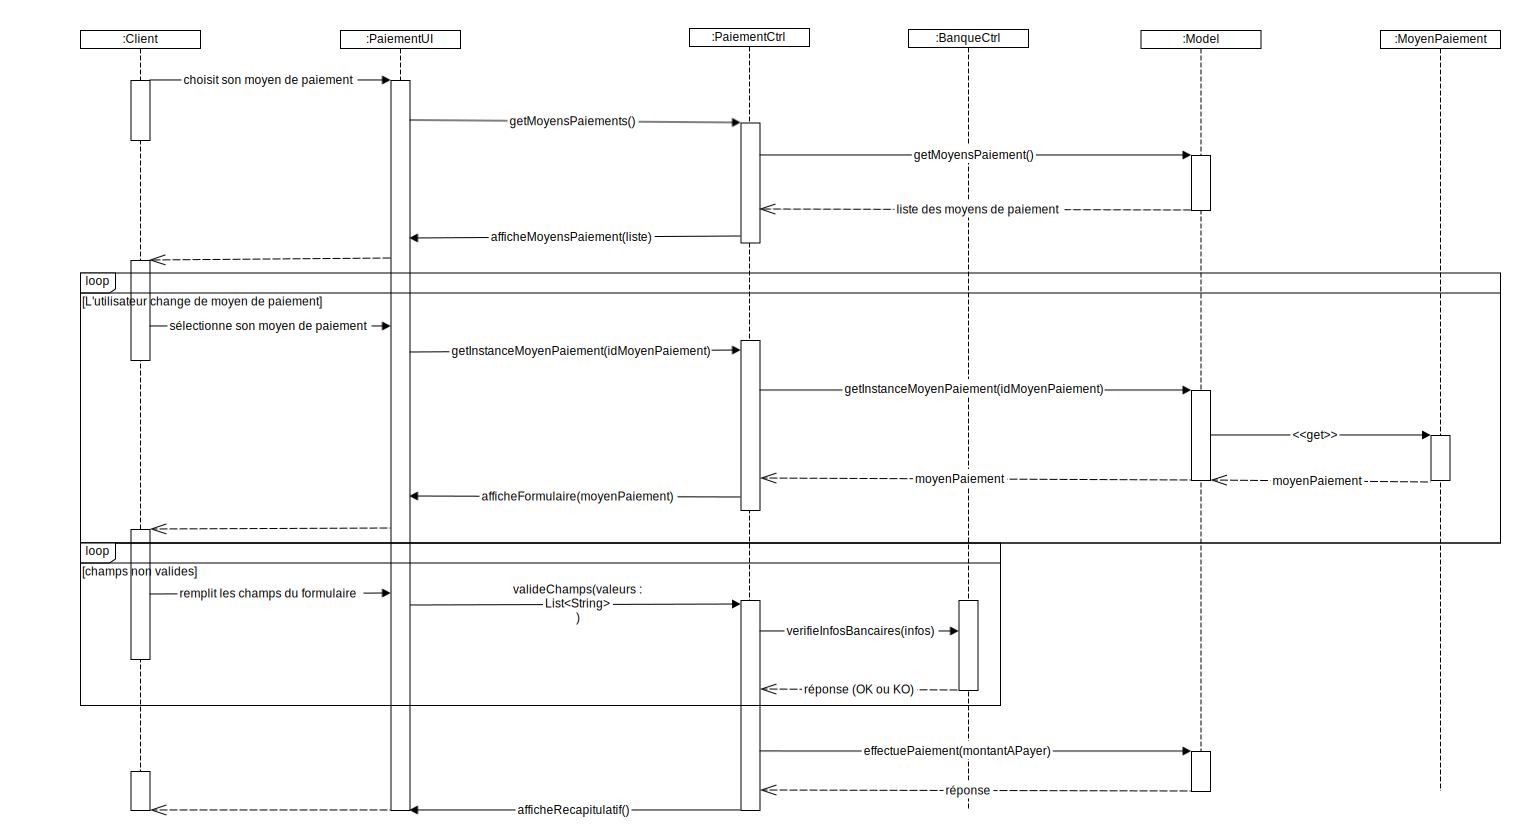
\includegraphics[height=8.5cm, width=\textwidth]{use_cases/pay.png}
	\subsubsection{Demander un \gls{robot}}
		~\\
		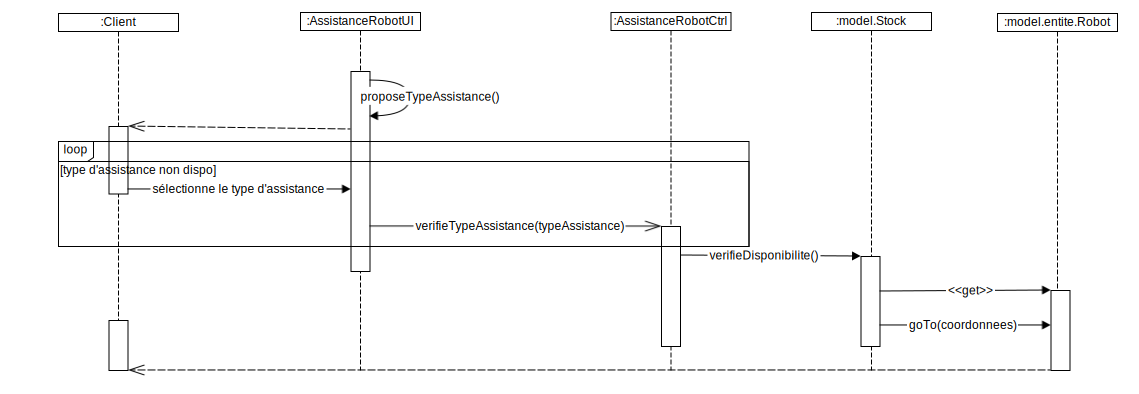
\includegraphics[height=7cm, width=\textwidth]{use_cases/robot_assistance.png}
	\subsubsection{Récupérer sa commande}
		~\\
		\includegraphics[height=6.5cm, width=\textwidth]{use_cases/retrieve_command.png}
			\subsection{Hiérarchie des cas d'utilisation}
	\newpage
			\newcolumntype{R}[1]{>{\raggedright\arraybackslash}p{#1}}
\newcolumntype{L}[1]{>{\raggedright\arraybackslash }b{#1}}
\newcolumntype{C}[1]{>{\raggedright\arraybackslash }b{#1}}
			\begin{longtable}{|R{5cm}|C{4cm}|L{4cm}|L{1cm}}
  \hline
  Cas d'utilisation & Utilisateur & Risque & Moyenne\\
  	\hline
	 RechercherArticle & 4 : Ne sera pas forcément utilisé si l’utilisateur connaît le magasin par exemple & 5 : plusieurs manières de rechercher : par photo, par QRCode, catégorie...Les technologies ne sont pas encore connues et maîtrisées de tous & 4.5 \\
	 \hline
	 ConsulterHistoriqueDAchat & 2: Cette fonctionnalité n’est pas primordiale. Il s’agit d’un plus pour l’utilisation de l’application & 1: L’historique d’achat de chaque utilisateur est stocké dans une base de donnée. Il suffit de faire une requete pour les récupérer. & 1.5\\
	 \hline
	 AjouterPanier & 5 : Primordial. L’utilisateur doit pouvoir ajouter des articles dans son panier virtuel pour pouvoir effectuer ses courses & 2 : Il suffit d’ajouter la référence de l’article et sa quantité dans notre liste
Vérifier au préalable en base que l’article est disponible en quantité suffisante & 3.5\\
	 \hline
	 ModifierPanier & 4 : Souvent l’utilisateur se trompe dans le choix de ses articles et il veut souvent modifier les articles qu’il a déjà sélectionnés. & 2: Il suffit de modifier une ligne d’article dans le panier ainsi que la base de donnée des articles. & 3\\
	 \hline
	 AssistanceRobot & 5 : Si un utilisateur vient dans notre magasin, c’est sûrement pour profiter de nos fonctionnalités novatrices & 4 : le robot intervient dans nos stocks et peut aider les utilisateurs (dans le magasin et/ou au chargement) & 4.5\\
	 \hline
	 Guidage & 4 : Les utilisateurs qui n’ont pas l’habitude de notre hypermarché auront forcément besoin du guidage pour se repérer & 5 : En plus de ne pas trop s’y connaître dans cette technologie, il nous faut maîtriser quelques algorithmes de plus court chemin (Ford Fulkerson, Dijkstra, Bellman ?), et pouvoir gérer le fait de capter le signal GPS à l’intérieur de l’hypermarché & 4.5\\
	 \hline
	 ValiderPanier & 4 : Ce sera la fonction qui permettra à l’utilisateur de confirmer ses achats, d’activer l’autoguidage vers la caisse et de passer au paiement. C’est une étape obligatoire. & 4: La validation du panier active beaucoup de fonctionnalités du système : le guidage, la préparation des commandes par les robots. & 4\\
	 \hline
	 Payer & 4 : Vital pour l’utilisateur; il doit payer ses articles & 5 : gérer les différentes manières de paiement et la sécurité (réseau lors de paiements à distance) & 4.5\\
	 \hline
	 RecupererCommande & 4 : très utile pour l’utilisateur; il choisira probablement la livraison ou le chargement par robot & 3 : affecter une commande à un type de livraison, pas de technologie particulière & 3.5\\
  	\hline
\end{longtable}
			\subsection{Description textuelle des cas d'utilisation}
	\subsubsection{RechercherArticleParCategorie}
	\underline{But} : Le client recherche un article sur l'application de son smartphone.\\
	\underline{Acteur principal} : Le client.\\
	\underline{Date de création} : 21/10/2014\\
	\underline{Responsable} : Groupe ASMA\\
	\underline{Version} : 1.0\\
	\underline{Déclenchement} : Le client sélection l'option "rechercher article par catégorie" dans son application.\\
	\underline{Pré-condition} : Le client est authentifié sur l'application fDrive.\\
	\underline{Séquence nominale} :
		\begin{enumerate}
			\item Le client sélectionne la catégorie d'articles qu'il désire consulter.
			\item Le système affiche la liste des articles concernés.
			\item Fin du cas d'utilisation.
		\end{enumerate}
	\underline{Post-condition} : Aucune.\\
	\underline{Scénario alternatif} : Aucun\\
	\underline{Scénario d'exception} :\\
 		1a [Le client annule sa recherche.]
 			\begin{enumerate}[label=1a.\arabic* ]
 				\item Le système prévient l'utilisateur.
 				\item Fin de la session.
 			\end{enumerate}
	\subsubsection{AjouterPanier}
	\underline{But} : Le client souhaite ajouter un article à sa commande courante à l'aide de l'application fDrive.\\
	\underline{Acteur principal} : Un client\\
	\underline{Date de création} : 21/10/2014\\
	\underline{Responsable} : Groupe ASMA\\
	\underline{Version} : 1.0\\
	\underline{Déclenchement} : Le client flashe/sélectionne un article dans l'application fDrive.\\
	\underline{Séquence nominale} :
		\begin{enumerate}
			\item Le système récupère la commande courante du client.
			\item Le système affiche un formulaire pour choisir la quantité désirée.
			\item Le client sélectionne la quantité désirée.
			\item Le système valide la quantité.
			\item Le système affiche l'ajout à la commande.
			\item Le système met à jour la commande courante du client.
			\item Fin du cas d'utilisation.
		\end{enumerate}
	\underline{Post-condition} : Un nouvel article est ajouté dans la commande courante du client.\\
	\underline{Scénario alternatif} :\\
		4a [La quantité est nulle.]
			\begin{enumerate}[label=4a.\arabic* ]
				\item Le système prévient l'utilisateur.
				\item Renvoie en 2.
			\end{enumerate}
	\underline{Scénario d'exception} :\\
		5a [Le client annule son ajout.]
			\begin{enumerate}[label=5a.\arabic* ]
				\item Le système prévient le client.
				\item Le système met fin à la session.
			\end{enumerate}
	\subsubsection{ModifierPanier}
	\underline{But} : Le client souhaite modifier un article de sa commande courante à l'aide de l'application fDrive.\\
	\underline{Acteur principal} : Un client.\\
	\underline{Date de création} : 21/10/2014\\
	\underline{Responable} : Groupe ASMA\\
	\underline{Version} : 1.0\\
	\underline{Déclenchement} : Le client sélectionne un article dans sa commande courante dans l'application fDrive.\\
	\underline{Pré-condition} : Le client est authentifié sur l'application fDrive.\\
	\underline{Séquence nominale} :
		\begin{enumerate}
			\item Le système affiche l’article sélectionné ainsi que la quantité.		
			\item Le système affiche un formulaire pour modifier l’article.
			\item Le système vérifie la modification.
			\item Le système affiche la modification.
			\item Le système met à jour la commande courante du client.
			\item Fin du cas d’utilisation.
		\end{enumerate}
	\underline{Post-condition} : La commande courante du client a été modifiée.\\
	\underline{Scénario alternatif} :\\
	 	3a [La quantité sélectionnée est inférieure à 0.]
		 	\begin{enumerate}[label=3a.\arabic* ]
		 		\item Le système prévient l'utilisateur.
		 		\item Fin de la session.
		 	\end{enumerate}
	\underline{Scénario d'exception} :\\
		2a [Le client supprime un article.]
			\begin{enumerate}[label=2a.\arabic* ]
				\item Le système prévient l'utilisateur.
				\item Le système supprime l'article de la commande courante.
				\item Le système met à jour la commande courante du client.
				\item Fin de la session.
			\end{enumerate}
		2b [Le client annule la modification de sa commande.]
			\begin{enumerate}[label=2b.\arabic* ]
				\item Le système prévient l'utilisateur.
				\item Fin de la session.
			\end{enumerate}
		3b [La quantité sélectionnée est égale à 0]
			\begin{enumerate}[label=3b.\arabic* ]
				\item Le système prévient l'utilisateur.
				\item Le système supprime l'article de la commande courante.
				\item Le système met à jour la commande courante du client.
				\item Fin de la session.
			\end{enumerate}
	\subsubsection{DemanderAssistanceRobot}
	\underline{But} : Un client demande l'assistance d'un robot pour une certaine tâche.\\
	\underline{Acteur principal} : Le client.\\
	\underline{Date de création} : 04/11/2014\\
	\underline{Responsable} : Groupe ASMA\\
	\underline{Version} : 1.0\\
	\underline{Déclenchement} : Le client sélectionne l'option "demander assistance robot" dans son application.\\
	\underline{Pré-condition} : Le client est authentifié sur l'application fDrive.\\
	\underline{Séquence nominale} :\\
		\begin{enumerate}
			\item Le client sélectionne le type d'assistance qu'il désire.
			\item Le système vérifie le type d'assistance.
			\item Le système vérifie la disponibilité des robots pour ce type d'assistance.
			\item Le système envoie un robot au client.
			\item Fin du cas d'utilisation.
		\end{enumerate}
	\underline{Post-condition} : Un robot est maintenant disponible pour utilisation.\\
	\underline{Scénarion alternatif} :\\
		2a [Le type d'assistance demandé n'est pas possible pour ce client.]
	 		\begin{enumerate}[label=2a.\arabic* ]
	 			\item Le système prévient l'utilisateur.
	 			\item Retour en 1.
	 		\end{enumerate}
		Note : Par exemple, un client ne peut pas demander une assistance robot pour charger ses courses dans son véhicule s'il n'a pas encore payé.\\
	\underline{Scénario d'exception} :\\
		1a [Le client annule sa demande d'assistance.]
			\begin{enumerate}[label=1a.\arabic* ]
	 			\item Le système prévient l'utilisateur.
	 			\item Fin de la session.
	 		\end{enumerate}
	 	3a [Aucun robot n'est disponible.]
	 		\begin{enumerate}[label=3a.\arabic* ]
	 			\item Le système prévient l'utilisateur.
	 			\item Fin de la session.
	 		\end{enumerate}
	\subsubsection{ValiderPanier}
	\underline{But} : Un client souhaite valider son panier afin de pouvoir payer et rentrer chez lui avec ses courses.\\
	\underline{Acteur principal} : Un client.\\
	\underline{Date de création} : 21/10/2014.\\
	\underline{Responsable} : Groupe ASMA\\
	\underline{Version} : 1.0\\
	\underline{Déclenchement} : Après avoir flashé/choisi les articles qu'il désire, le client choisit de valider son panier à l'aide de l'application fDrive.\\
	\underline{Pré-condition} : Le client est authentifié sur l'application fDrive.\\
	\underline{Séquence nominale} :
		\begin{enumerate}
			\item Le système récupère la liste des articles sélectionnés par le client.
			\item Le système vérifie les disponibilités de ces articles.
			\item Le système demande la confirmation au client avant de valider.
			\item Le système affecte la commande à une caisse.
			\item Le système affiche le numéro de caisse et le numéro de commande associé à la commande du client.
			\item Le système propose l'auto-guidage vers cette caisse.
			\item Fin du cas d'utilisation.
		\end{enumerate}
	\underline{Post-condition} : Le système est en attente d'un paiement pour cette commande.\\
	\underline{Scénario alternatif} :\\
		2a. [Un article n'est plus disponible.]
			\begin{enumerate}[label=2a.\arabic* ]
				\item Le système prévient le client.
				\item Le système propose des articles similaires disponibles.
				\item Le client choisit un articles de remplacement ou valide sans cet article.
				\item Le système met à jour la commande.
				\item Renvoie en 2.
			\end{enumerate}
		2b. [La quantité disponible est insuffisante.]
			\begin{enumerate}[label=2b.\arabic* ]
	       		\item Le système prévient le client.
				\item Le système propose la quantité maximale disponible.
				\item Le client choisit une quantité ou valide sans cet article..
				\item Le système met à jour la commande.
				\item Renvoie en 2.
			\end{enumerate} 
	\underline{Scenario d’exception} :\\
		1a [La commande est vide.]
			\begin{enumerate}[label=1a.\arabic* ]
				\item Le système prévient l'utilisateur.
				\item Le système met fin à la session.
			\end{enumerate}
		3a [Le client ne confirme pas sa commande.]
			\begin{enumerate}[label=3a.\arabic* ]
				\item Le système prévient l'utilisateur.
				\item Le système met fin à la session.
			\end{enumerate}
	\subsubsection{Paiement}
	\underline{But} : Le client désire payer.\\
	\underline{Acteur principal} : Le client.\\
	\underline{Date de création} : 04/11/2014\\
	\underline{Responsable} : Groupe ASMA\\
	\underline{Version} : 1.0\\
	\underline{Déclenchement} : Le client se trouve à la caisse indiquée par l'application lors de la validation de son panier.\\
	\underline{Pré-condition} : Le client doit être authentifié.\\
	\underline{Séquence nominale} :
		\begin{enumerate}
			\item Le client sélectionne le moyen de paiement désiré.
			\item Le système affiche les instructions à suivre afin de payer.
			\item Le système vérifie le paiement du client.
			\item Le système donne au client sa commande préparé par les robots de stocks.
			\item Fin du cas d'utilisation.
		\end{enumerate}
	\underline{Post-condition} : Le panier du client est payé.\\
	\underline{Scénario alternatif} :\\
		2a [Le client change de moyen de paiement.]
	 		\begin{enumerate}[label=2a.\arabic* ]
	 			\item Le système prévient l'utilisateur.
	 			\item Retour en 1.
 			\end{enumerate}
		3a [Le client n'a pas bien suivi les instructions de paiement.]
 			\begin{enumerate}[label=3a.\arabic* ]
 				\item Le système prévient l'utilisateur.
 				\item Retour en 2.
 			\end{enumerate}
	 \underline{Scénario d'exception} :\\
	 	1a [Le client annule son paiement]
	 		\begin{enumerate}[label=1a.\arabic* ]
	 			\item Le système prévient l'utilisateur.
	 			\item Retour en 1.
	 		\end{enumerate}

			\subsection{Maquettes de l'application mobile}
	\subsubsection{Accueil}
		~\\
		\includegraphics[height=20cm]{models/home.png}
	\subsubsection{Menu principal}
		~\\
		\includegraphics[height=20cm]{models/menu.png}
	\subsubsection{Rechercher un article}
		~\\
		\includegraphics[height=20cm]{models/search.png}
	\subsubsection{Ajouter un article au panier}
		~\\
		\includegraphics[height=20cm]{models/add_article.png}
	\subsubsection{Promotions du magasin}
		~\\
		\includegraphics[height=20cm]{models/promotions.png}
	\subsubsection{Navigation vers un rayon}
		~\\
		\includegraphics[height=20cm]{models/shelf_navigation.png}
	\subsubsection{Historique des achats}
		~\\
		\includegraphics[height=20cm]{models/purchase_history.png}
	\subsubsection{Guidage/Navigation}
		~\\
		\includegraphics[height=20cm]{models/mapping.png}
	\subsubsection{Voir panier}
		~\\
		\includegraphics[height=20cm]{models/cart.png}
	\subsubsection{Récapitulation de la commande}
		~\\
		\includegraphics[height=20cm]{models/recapitulation.png}
			\subsection{Modèles d'objets}
	\subsubsection{Vue d'ensemble}
		\includegraphics{}
			\subsection{Modèles dynamiques}
				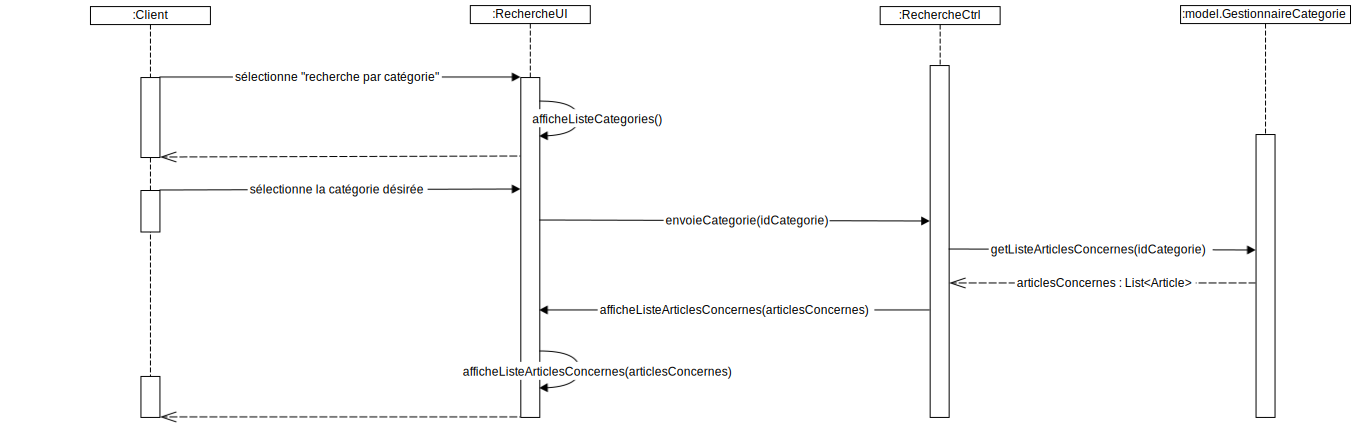
\includegraphics[width=\textwidth]{sequence_diagrams/search_by_category.pdf}
	
	\glossarystyle{listgroup}
	\pagestyle{glossary}
	\printglossary[title=Glossaire métier,toctitle=Glossaire métier]
	
	\chapter*{Références/bibliographie}
		\url{http://wikipedia.org} \\
		\url{http://larousse.fr} \\

\end{document}